\chapter{Einleitung}
% Hier folgt eine kurze Einleitung in die Thematik der Bachelorarbeit.
% Die Einleitung muss kurz sein, damit die vorgegebene Gesamtlänge der 
% Arbeit von 25 Seiten nicht überschritten wird. 
% Die Beschränkung der Seitenzahl sollte man ernst nehmen,
% da Überschreitung zu Abzügen in der Note führen kann. 
% Um der Längenbeschränkung zu genügen, darf auch nicht an der Schriftgröße,
% dem Zeilenabstand oder dem Satzspiegel (bedruckte Fläche der Seite) manipuliert werden.


The IceCube neutrino detector is a cubic kilometer scale particle detector located near the Amundsen-Scott South Pole Station. The primary goal of 
the detector is the detection of high energy neutrinos as messenger particles for study of astrophysical sources. The detector unit is split into three 
parts, which are the In-Ice Array, the IceTop, and the DeepCore. 

The In-Ice Array is the largest component and consists of 86 vertical strings, extending vertically into the ice below the surface for \SI{1450}{\metre} 
to \SI{2450}{\metre}. Each of the strings contains 60 Digital Optical Modules (DOMs) which are evenly separated by \SI{17}{\metre} alongside their 
respective string, making a total number of \num{5160} DOMs. 

The IceTop, as the name suggests, in located at the surface of the ice with \num{162} tanks filled with ice and equipped with PMTs. 
The tanks are arranged in 81 stations in a manner that approximately mimics the structure of the In-Ice Array. 

The DeepCore is a sub-array within the In-Ice Array and is located at depth beneath \SI{1750}{\metre}.It contains an extra \num{8} strings alongside the 
\num{7} strings from the In-Ice Array. This creates a more densly packed arrangement of DOMs in the lower center of the detector, which increases it's 
ability to detect low-energy signals.

Figure~\ref{fig:icecube_sketch_01} shows a visual representation of this structure.

\begin{figure}[htbp]
    \centering
    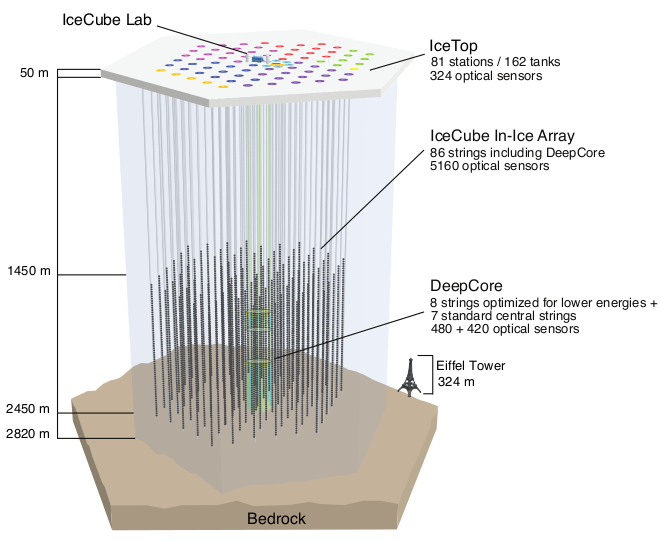
\includegraphics[width=\textwidth]{content/pictures/icecube_sketch_01.png}
    \caption{An overview of the arrangement inside of the detector.}\label{fig:icecube_sketch_01}
\end{figure}

\section{Digital Optical Module}

A single DOM consists of a glass housing, in which the PMT and the corresponding curcuit boards are located. The technical part of the functionality of 
the circuit boards are not of interest for this analysis, so I will not go into detail on that topic. The PMT however is the actual detecting unit of 
the DOM\. A sketch of a PMT is shown in figure~\ref{fig:pmt01}.

\begin{figure}[htbp]
    \centering
    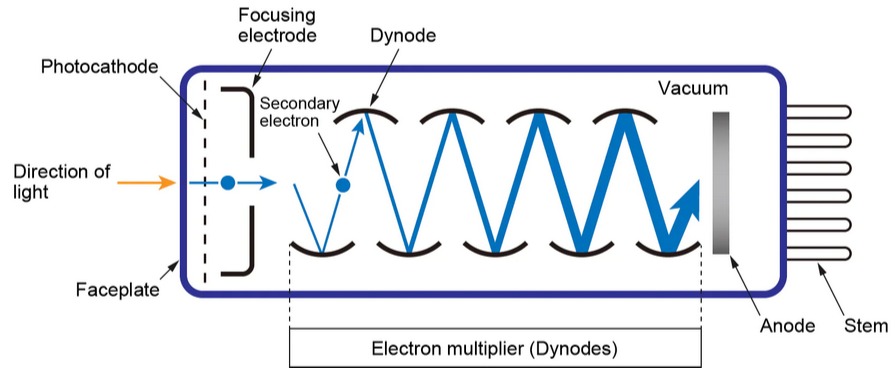
\includegraphics[width=\textwidth]{content/pictures/pmt_sketch_01.png}
    \caption{The principle construction of a photomultiplier.}\label{fig:pmt01}
\end{figure}

When a photon with sufficient energy hits the photocathode of the PMT, it's energy gets absorbed and an electron is emitted via the photoelectric effect.
the electron is accelerated towards the first dynode due to its electric charge. Hitting the dynode triggers secondary emittions, increasing the total 
number of electrons emitted. This process repeats itself for however many dynodes are the PMT accompasses. After the final amplification by the last 
dynode the electrons are collected by the anode, which produces a current proportional to the intensity of the initial light signal, meaning the amount of
photons hitting the PMT\@. 

\section{Cherenkov radiation}

The light detected by the photomultipliers is only a secondary signal called Cherenkov radiation. It is created when a charged particle travels through a 
dielectric medium with a velocity greater than the speed of light inside of the medium. The charged particle polarizes the medium's molecules in it's
immediate surroundings while passing through it. The excited molecules then return to their ground state by emitting their superfluous energy as light.
Because the light travels slower than the particle exciting the molecules, the light waves do not interfere destructively, but build a conical shock front 
similar in principle to that of an object, moving through air at supersonic velocities. 
